\documentclass[12pt]{article}
\usepackage[utf8]{inputenc}
\usepackage{amsmath, amssymb}
\usepackage{xcolor}
\usepackage{geometry}
\usepackage{hyperref}
\usepackage{fancyhdr}
\usepackage{enumitem}
\usepackage{graphicx}
\usepackage{booktabs}
\usepackage{tikz}
\usetikzlibrary{shapes,arrows,positioning,fit, arrows.meta}

\geometry{margin=1in}
\hypersetup{colorlinks=true, linkcolor=blue, urlcolor=cyan}

\pagestyle{fancy}
\fancyhf{}
\fancyhead[L]{\textbf{\TOPICTITLE}}
\fancyhead[R]{\thepage}




% -------------------------------
% Topic Metadata
% -------------------------------
\newcommand{\TOPICTITLE}{Application Layer: E-mail, SMTP, and IMAP_s}
\title{\TOPICTITLE\\\large Study-Ready Notes}
\author{Andrew Photinakis}
\date{\today}

\setlength{\headheight}{15pt}

\begin{document}
\maketitle
\tableofcontents


\newpage

% This LaTeX file should be saved at: computer_networks/week05/application_layer_email_smtp_imap.tex

\section{Introduction to Application Layer}
\begin{itemize}
    \item Application layer is the top layer in network protocol stack
    \item Provides services directly to user applications
    \item Key protocols: HTTP, SMTP, IMAP, DNS
    \item Socket programming enables application development
\end{itemize}

\textcolor{blue}{[Summary: The application layer serves as the interface between network services and user applications, implementing protocols like HTTP for web, SMTP for email, and DNS for name resolution.]}

\section{E-mail Infrastructure}

\subsection{Three Major Components}
\begin{enumerate}
    \item \textbf{User Agents}
          \begin{itemize}
              \item Also known as "mail readers"
              \item Functions: composing, editing, reading mail messages
              \item Examples: Outlook, iPhone mail client
              \item Stores outgoing and incoming messages on server
          \end{itemize}

    \item \textbf{Mail Servers}
          \begin{itemize}
              \item Contains user mailboxes for incoming messages
              \item Maintains message queue for outgoing mail
              \item Multiple servers communicate via SMTP
          \end{itemize}

    \item \textbf{Simple Mail Transfer Protocol (SMTP)}
          \begin{itemize}
              \item Protocol for transferring email between servers
              \item Uses TCP for reliable delivery
              \item Operates on port 25
          \end{itemize}
\end{enumerate}

\subsection{E-mail Architecture Diagram}
\begin{figure}[h]
    \centering
    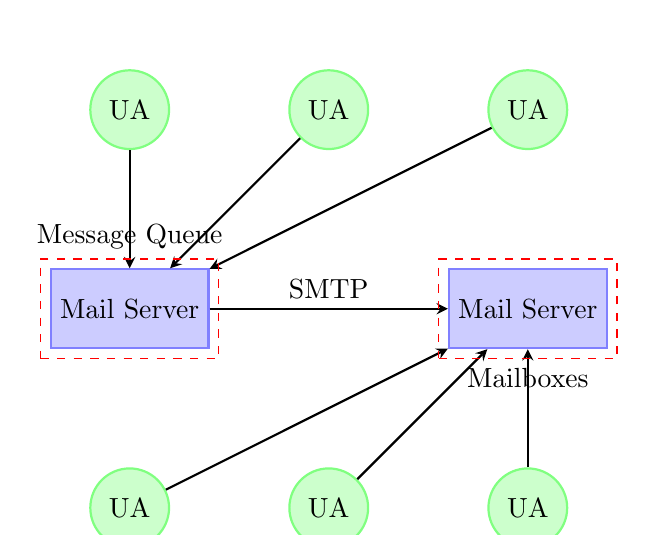
\begin{tikzpicture}[
            node distance=1.5cm,
            server/.style={rectangle, draw=blue!50, fill=blue!20, thick, minimum width=2cm, minimum height=1cm},
            agent/.style={circle, draw=green!50, fill=green!20, thick, minimum size=1cm},
            protocol/.style={->, >=stealth, thick}
        ]

        \node[agent] (ua1) {UA};
        \node[agent] (ua2) [right=of ua1] {UA};
        \node[agent] (ua3) [right=of ua2] {UA};

        \node[server] (server1) [below=of ua1] {Mail Server};
        \node[server] (server2) [below=of ua3] {Mail Server};

        \node[agent] (ua4) [below=of server1] {UA};
        \node[agent] (ua5) [right=of ua4] {UA};
        \node[agent] (ua6) [right=of ua5] {UA};

        \draw[protocol] (ua1) -- (server1);
        \draw[protocol] (ua2) -- (server1);
        \draw[protocol] (ua3) -- (server1);
        \draw[protocol] (ua4) -- (server2);
        \draw[protocol] (ua5) -- (server2);
        \draw[protocol] (ua6) -- (server2);
        \draw[protocol] (server1) -- node[above] {SMTP} (server2);

        \node[draw=red, dashed, fit=(server1), label=above:Message Queue] {};
        \node[draw=red, dashed, fit=(server2), label=below:Mailboxes] {};

    \end{tikzpicture}
    \caption{E-mail system architecture showing user agents (UA), mail servers, and SMTP protocol flow}
\end{figure}

\textcolor{orange}{[Mnemonic: USA - User agents, Servers, SMTP Architecture]}
\textcolor{blue}{[Summary: Email infrastructure consists of user agents for interface, mail servers for storage and queuing, and SMTP protocol for server-to-server communication.]}



\section{Simple Mail Transfer Protocol (SMTP)}

\subsection{SMTP Protocol Overview}
\begin{itemize}
    \item Defined in RFC 5321
    \item Uses TCP for reliable transfer on port 25
    \item Direct transfer: sending server acts as client to receiving server
    \item Three-phase transfer process:
          \begin{enumerate}
              \item SMTP handshaking (greeting)
              \item SMTP transfer of messages
              \item SMTP closure
          \end{enumerate}
    \item Command/response interaction using ASCII text
\end{itemize}

\subsection{SMTP Session Timeline}
\begin{figure}[h]
    \centering
    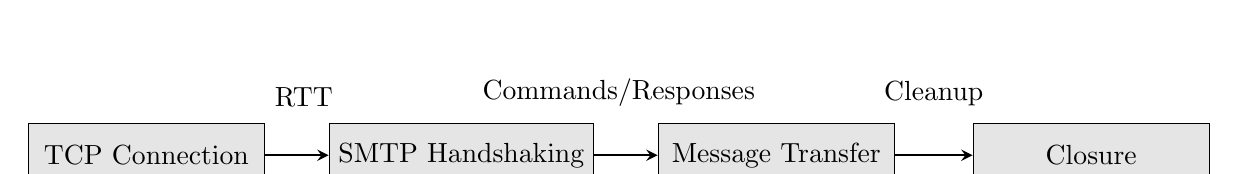
\begin{tikzpicture}[
            timeline/.style={->, >=stealth, thick},
            phase/.style={rectangle, draw=black, fill=gray!20, minimum width=3cm, minimum height=0.8cm}
        ]

        \node[phase] (tcp) at (0,0) {TCP Connection};
        \node[phase] (handshake) at (4,0) {SMTP Handshaking};
        \node[phase] (transfer) at (8,0) {Message Transfer};
        \node[phase] (closure) at (12,0) {Closure};

        \draw[timeline] (tcp) -- (handshake);
        \draw[timeline] (handshake) -- (transfer);
        \draw[timeline] (transfer) -- (closure);

        \node[above] at (2,0.5) {RTT};
        \node[above] at (6,0.5) {Commands/Responses};
        \node[above] at (10,0.5) {Cleanup};

    \end{tikzpicture}
    \caption{SMTP protocol phases showing the sequence of operations during email transfer}
\end{figure}

\subsection{Email Delivery Scenario: Alice to Bob}
\begin{enumerate}
    \item Alice uses UA to compose email to bob@someschool.edu
    \item Alice's UA sends message to her mail server using SMTP
    \item Message placed in outgoing message queue
    \item SMTP client at Alice's server opens TCP connection with Bob's server
    \item SMTP client sends Alice's message over TCP connection
    \item Bob's server places message in Bob's mailbox
    \item Bob uses UA to read message via mail access protocol
\end{enumerate}

\textcolor{teal}{[Concept Map: User Agent → Outgoing Server → SMTP → Incoming Server → Mailbox → User Agent]}

\section{SMTP Protocol Details}

\subsection{Sample SMTP Interaction}
\begin{verbatim}
S: 220 hamburger.edu
C: HELO crepes.fr
S: 250 Hello crepes.fr, pleased to meet you
C: MAIL FROM: <alice@crepes.fr>
S: 250 alice@crepes.fr... Sender ok
C: RCPT TO: <bob@hamburger.edu>
S: 250 bob@hamburger.edu ... Recipient ok
C: DATA
S: 354 Enter mail, end with "." on a line by itself
C: Do you like ketchup?
C: How about pickles?
C: .
S: 250 Message accepted for delivery
C: QUIT
S: 221 hamburger.edu closing connection
\end{verbatim}

\subsection{SMTP Observations and Comparisons}

\subsubsection{Comparison with HTTP}
\begin{table}[h]
    \centering
    \begin{tabular}{p{6cm}p{6cm}}
        \toprule
        \textbf{SMTP}                         & \textbf{HTTP}                            \\
        \midrule
        Client push protocol                  & Client pull protocol                     \\
        ASCII command/response interaction    & ASCII command/response interaction       \\
        Multiple objects in multipart message & Each object in separate response message \\
        Persistent connections                & Both persistent and non-persistent       \\
        7-bit ASCII requirement for messages  & No encoding restrictions                 \\
        CRLF.CRLF marks end of message        & Content-Length or chunked encoding       \\
        \bottomrule
    \end{tabular}
    \caption{Comparison between SMTP and HTTP protocols}
\end{table}

\subsubsection{Key SMTP Characteristics}
\begin{itemize}
    \item \textbf{Push Protocol}: Sending server initiates transfer
    \item \textbf{7-bit ASCII}: Messages must be in 7-bit ASCII format
    \item \textbf{Persistent Connections}: Multiple messages can be sent in single connection
    \item \textbf{Message Delimiter}: CRLF.CRLF indicates end of message
\end{itemize}

\textcolor{blue}{[Summary: SMTP uses a push model with persistent connections, requires 7-bit ASCII encoding, and follows a strict command-response sequence for reliable email transfer between servers.]}

\section{Mail Message Format}

\subsection{RFC Standards}
\begin{itemize}
    \item \textbf{RFC 5321}: Defines SMTP protocol (equivalent to RFC 7231 for HTTP)
    \item \textbf{RFC 2822}: Defines syntax for email message format (equivalent to HTML for web)
\end{itemize}

\subsection{Message Structure}
\begin{verbatim}
Header
To: bob@hamburger.edu
From: alice@crepes.fr
Subject: Lunch plans

Body
Let's meet at the usual place at noon.
.
\end{verbatim}

\subsubsection{Header Fields}
\begin{itemize}
    \item \textbf{To}: Recipient's email address
    \item \textbf{From}: Sender's email address
    \item \textbf{Subject}: Brief description of message content
    \item Note: These are different from SMTP commands MAIL FROM and RCPT TO
\end{itemize}

\subsubsection{Body Format}
\begin{itemize}
    \item Contains the actual message content
    \item Originally ASCII characters only
    \item Separated from headers by blank line
\end{itemize}

\textcolor{orange}{[Mnemonic: HBS - Headers, Blank line, Body Structure]}

\section{Mail Access Protocols}

\subsection{Email Retrieval Architecture}
\begin{figure}[h]
    \centering
    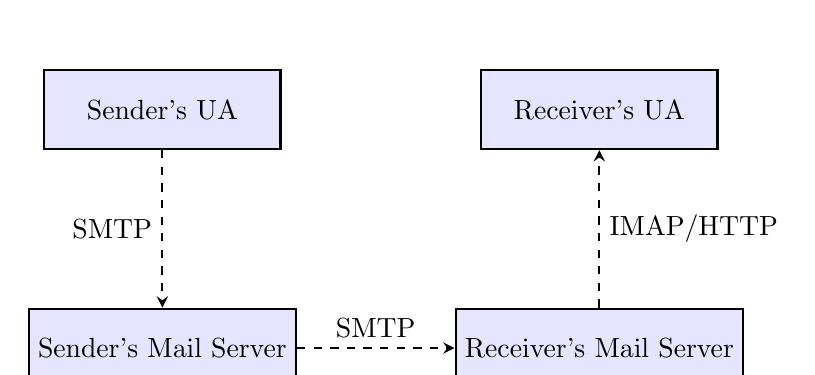
\begin{tikzpicture}[
            node distance=2cm,
            component/.style={rectangle, draw=black, fill=blue!10, thick, minimum width=3cm, minimum height=1cm},
            protocol/.style={->, >=stealth, thick, dashed}
        ]

        \node[component] (sender) {Sender's UA};
        \node[component] (senderserver) [below=of sender] {Sender's Mail Server};
        \node[component] (receiverserver) [right=of senderserver] {Receiver's Mail Server};
        \node[component] (receiver) [above=of receiverserver] {Receiver's UA};

        \draw[protocol] (sender) -- node[left] {SMTP} (senderserver);
        \draw[protocol] (senderserver) -- node[above] {SMTP} (receiverserver);
        \draw[protocol] (receiverserver) -- node[right] {IMAP/HTTP} (receiver);

    \end{tikzpicture}
    \caption{Email flow showing SMTP for delivery and access protocols for retrieval}
\end{figure}

\subsection{Mail Access Protocols}
\begin{itemize}
    \item \textbf{SMTP}: Used for delivery and storage to receiver's server
    \item \textbf{Mail Access Protocols}: Used for retrieval from server to user agent
\end{itemize}

\subsubsection{IMAP (Internet Mail Access Protocol)}
\begin{itemize}
    \item Defined in RFC 3501
    \item Messages stored on server
    \item Provides retrieval, deletion, and folder management
    \item Maintains messages on server after reading
\end{itemize}

\subsubsection{HTTP-based Email}
\begin{itemize}
    \item Used by webmail services: Gmail, Hotmail, Yahoo!Mail
    \item Web-based interface on top of SMTP (sending) and IMAP/POP (retrieval)
    \item Provides rich user interface through web browser
\end{itemize}

\textcolor{blue}{[Summary: While SMTP handles server-to-server delivery, mail access protocols like IMAP and HTTP handle retrieval from servers to user agents, with IMAP maintaining server storage and HTTP providing web interfaces.]}

\section{Key Concepts Review}

\subsection{Important Definitions}
\begin{itemize}
    \item \textbf{User Agent}: Mail client software for composing, reading, and managing email
    \item \textbf{Mailbox}: Storage area on mail server for incoming user messages
    \item \textbf{Message Queue}: Temporary storage for outgoing messages awaiting transfer
    \item \textbf{SMTP}: Application layer protocol for reliable email transfer between servers
    \item \textbf{IMAP}: Protocol for accessing and managing email on remote servers
\end{itemize}

\subsection{Protocol Comparison Summary}
\begin{itemize}
    \item \textbf{SMTP}: Push protocol, server-to-server, port 25, 7-bit ASCII
    \item \textbf{IMAP}: Pull protocol, server-to-client, port 143, server storage
    \item \textbf{HTTP}: Pull protocol, web interface, ports 80/443, rich content
\end{itemize}

\textcolor{teal}{[Concept Map: Email Flow: Composition → UA → SMTP → Server Queue → SMTP → Receiver Server → Mailbox → Access Protocol → UA → Reading]}

\section{Study Aids}

\subsection{Mnemonics}
\begin{itemize}
    \item \textcolor{orange}{USA}: User agents, Servers, SMTP Architecture
    \item \textcolor{orange}{HBS}: Headers, Blank line, Body Structure
    \item \textcolor{orange}{PPS}: Push (SMTP) vs Pull (HTTP/IMAP) Services
\end{itemize}

\subsection{Key Points to Remember}
\begin{itemize}
    \item SMTP is used between mail servers, not between user agent and server
    \item Email has two types of addressing: SMTP commands and message headers
    \item IMAP keeps messages on server, POP3 typically downloads to local machine
    \item HTTP-based email adds web interface layer to traditional email protocols
\end{itemize}

\end{document}